\mychapter{3}{Input variable analysis}
\label{sec:unchapitre}

A large set of variables is available from CMS data. MVA training can be time consumming and the "curse of
dimensionality"(1) forces us to select only a few of them based on two main criteria :
\begin{description}
    \item [Background vs Signal discrimination :] Variables with most differences of shape for background and signal will be picked.
    \item [Low correlation between variables :] Needed in order to reduce redundancy of input data and thus will permit
    to reduce MVA complexity (for example number of hidden neurons in ANN).
\end{description}

reference \cite{CMS2015}.

\section{Background vs Signal discrimination}

It is necessary to pick the smallest set of input variable for the MVA. This selection is done by looking at variable
shape for background and signal data from MC simulation. (fig. \ref{NHiso_photon_dataVsMCbg})

\begin{figure}[h!]
  \centering
  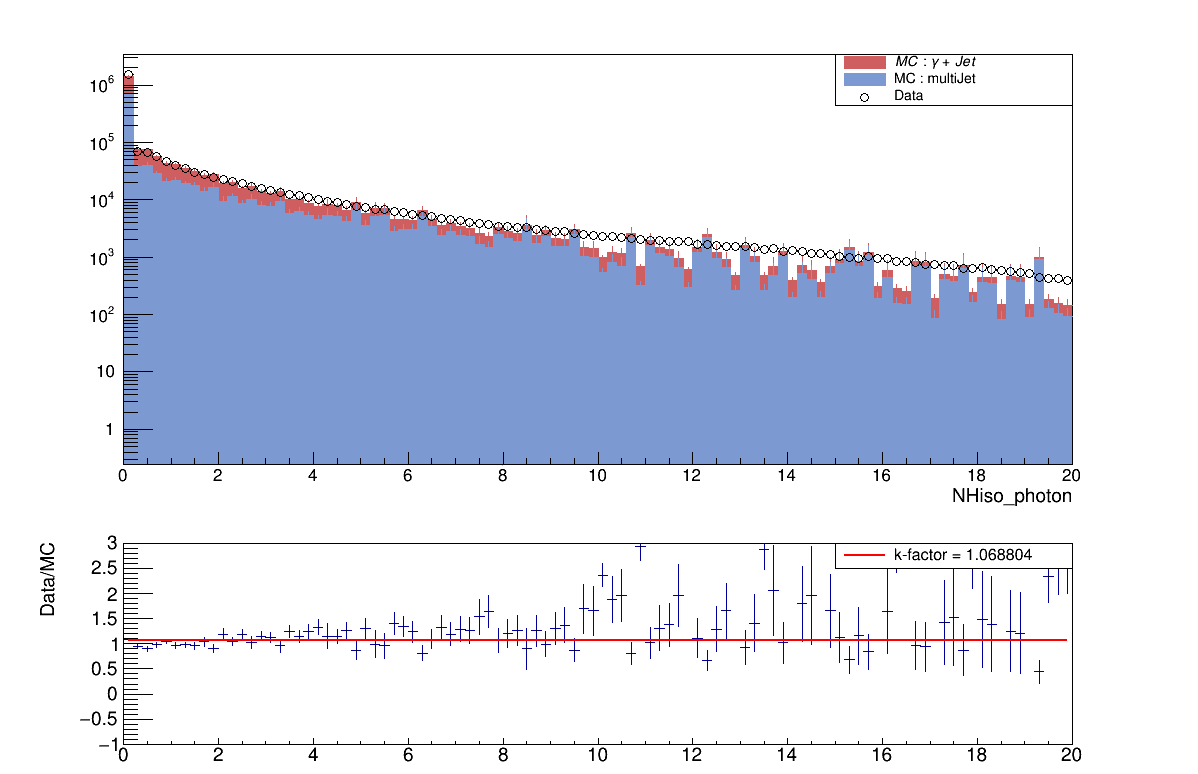
\includegraphics[width=0.8\textwidth]{NHiso_photon}\\[1cm]
  \caption{Neutral hadron isolation for background and signal MC}
  \label{NHiso_photon_dataVsMCbg}
\end{figure}


\section{Variable correlations}

Training data needed-quantity increases with network complexity. So correlation between variables must be avoided in
order to get the minimum redundancy. By looking at the correlation matrix (fig. \ref{corrMatrix_bgMC}) we can see that CHiso is
a good candidate and so will be used next for the background estimation.

\begin{figure}[h!]
  \centering
  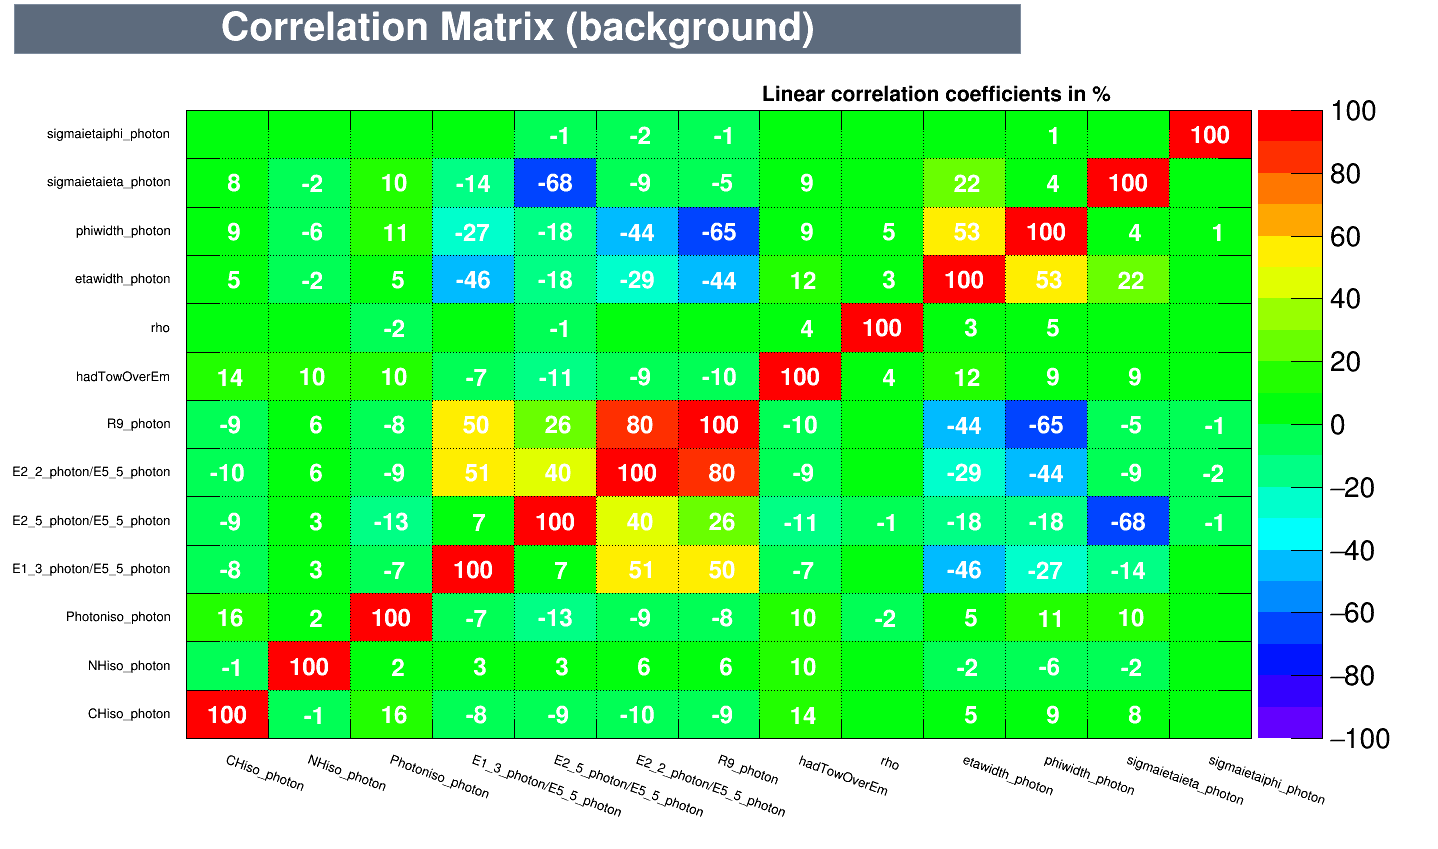
\includegraphics[width=0.8\textwidth]{corrMatrix_bgMC}\\[1cm]
  \caption{Correlation matrix for background MC}
  \label{corrMatrix_bgMC}
\end{figure}

\section{Data driven background estimation}

MVA will be performed with real data for the background, thereby a sideband (fig. \ref{sideband}) has to be defined on a low-correlated
variable that won't be used in the MVA. MC simulations allow us to estimate the signal purity after applying a cut on CHiso.

\begin{figure}[h!]
  \centering
  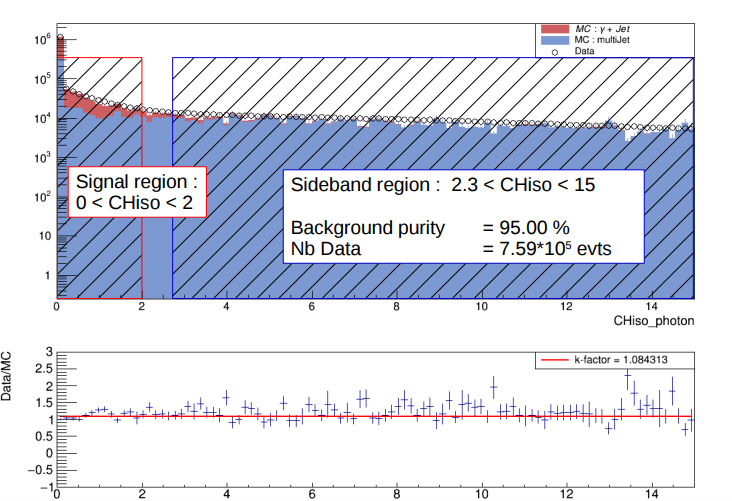
\includegraphics[width=0.8\textwidth]{sideband}\\[1cm]
  \caption{Charged hadron isolation for background and signal MC (histograms), signal region (red shaded area) and
  sideband (blue shaded area).}
  \label{sideband}
\end{figure}

Then we compare variables shape for background MC and DATA in the sideband region (fig. \ref{MCbg_all_NHiso_photon})

\begin{figure}[h!]
  \centering
  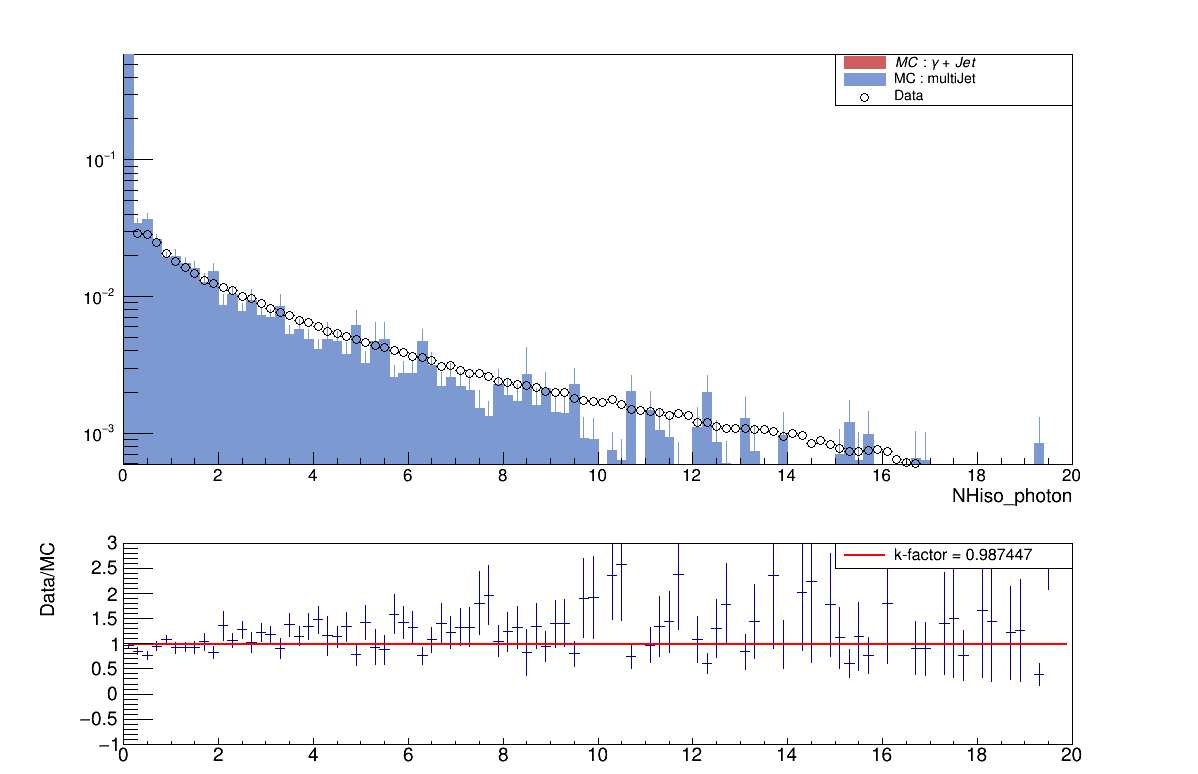
\includegraphics[width=0.8\textwidth]{MCbg_all_NHiso_photon}\\[1cm]
  \caption{Neutral hadron isolation for background MC and DATA in the sideband region}
  \label{MCbg_all_NHiso_photon}
\end{figure}

%%% Local Variables: 
%%% mode: latex
%%% TeX-master: "isae-report-template"
%%% End: 
